A partir de la gráfica de la figura \ref{fig:SINMAT1_U3_AC75_IMG3} que registra el cambio de temperatura con respecto al tiempo, de una muestra de agua a la que se aplica una cantidad constante de calor, escribe la cantidad correcta en el cuadro de texto.

\begin{multicols}{2}
    \begin{figure}[H]
        \centering
        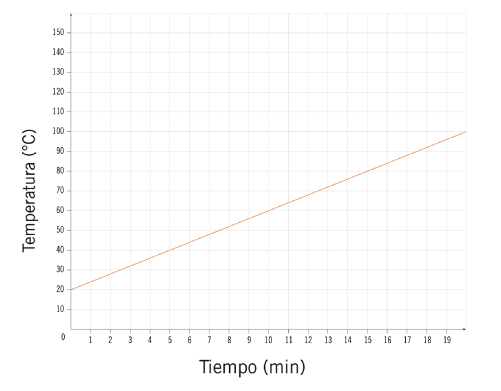
\includegraphics[width=0.8\linewidth]{../images/SINMAT1_U3_AC75_IMG3.jpg}
        \caption{Gráfica de la temperatura conforme pasa el tiempo.}
        \label{fig:SINMAT1_U3_AC75_IMG3}
    \end{figure}
    \begin{parts}
       \part \include*{../parts/question075c01}
       \part \include*{../parts/question075c02}
       \part \include*{../parts/question075c03}
       \part \include*{../parts/question075c04}
       \part \include*{../parts/question075c05}
    \end{parts}
\end{multicols}